\documentclass[12pt,a4paper]{report}
\usepackage[utf8]{inputenc}
\usepackage{amsmath}
\usepackage{amssymb}
\usepackage{caption}
\usepackage{fancyhdr}
\usepackage{float}
\usepackage{graphicx}
\usepackage{hyperref}
\usepackage{subcaption}
\usepackage[svgnames]{xcolor}

\newcommand*{\titleBC}{
	\begingroup
	\centering

	\def\CP{\textit{\Large Simulating argon}}

	\settowidth{\unitlength}{\CP} % Set the width of the curly brackets to the width of the title
	{\color{CadetBlue}\resizebox*{\unitlength}{\baselineskip}{\rotatebox{90}{$\}$}}} \\[\baselineskip] % Print top curly bracket
	{\color{Black}{\CP}} \\[\baselineskip] % Print title
	{\color{Black}\large Computational Physics} \\
	{\color{Grey}\large Delft University of Technology} \\
	{\color{CadetBlue}\resizebox*{\unitlength}{\baselineskip}{\rotatebox{-90}{$\}$}}} % Print bottom curly bracket
	\vfill
	\large{\textbf{Ludwig Rasmijn (4106644)}}\\
	\large{\textbf{Sebastiaan Lokhorst (4005058)}}\\
	\large{\textbf{Shang-Jen Wang (4215974)}}\\
	\vfill
	\pagestyle{empty}
	27 February 2015

	\endgroup
}

\begin{document}

\pagestyle{empty}
\pagenumbering{gobble}
\titleBC

\newpage

\begin{abstract}
We have created a molecular dynamics simulation to investigate the behavior of a homogeneous system of e.g. argon particles. In our simulation, the particles interact with a Lennard-Jones potential. The velocity Verlet algorithm is used to integrate the equations of motion and update the position and velocity of the particles. The initial conditions consist of the particles spaced out evenly in a FCC lattice, with an initial velocity drawn from the Maxwell-Boltzman distribution as a function of the initial temperature. We use periodic boundary conditions to only simulate the interaction between argon atoms.

After verifying that all basic laws such as energy conservation hold, we have investigated multiple properties. We have determined the specific heat of the system at multiple densities and our results were in accordance with previous simulations and experiments. Besides that we have also investigated the phase of our system at various temperatures and densities by computing the spacial correlation of the particles and looking at the compressibility of the system. The spacial correlation clearly shows the difference between a gas, fluid or solid phase. This was also noticeable when looking at isothermal lines in a compression diagram.
\end{abstract}

\newpage

\tableofcontents

\newpage

\pagestyle{fancy}
% Clear the header and footer
\fancyhead{}
\fancyfoot{}
\renewcommand{\headrulewidth}{0pt}
% Set the right side of the footer to be the page number
\fancyfoot[C]{\thepage}
\pagenumbering{arabic}

\chapter{Introduction}

Using statistical physics, a lot of properties of a system can be derived by looking at the behavior of many particles. Because direct experimentation is impossible, it is an ideal subject to simulate in a computer program. Starting out with the right inter-particle potential, one can simulate the interaction and movement of the particles. Combined with the right initial and boundary conditions, it is possible to determine some thermodynamical properties of a material like the temperature, spacial correlation, pressure and diffusion.

\chapter{Theory}

In order to simulate argon four questions have to be answered, these are:
\begin{enumerate}
 \item What is the interaction between the argon atoms?
 \item How do the argon atoms move around?
 \item What are the boundary conditions?
 \item What are the initial conditions?
\end{enumerate}
These will be answered in the following sections.\\ \\
The simulation can be verified by looking at a few properties of the argon interaction.\\ In this report pressure, specific heat, correlation function and diffusion constant are calculated in order to verify the correctness of the simulation.

\section{Lennard-Jones potential}

In this section the question ``What is the interaction between the argon atoms?" will be answered.\\
A simple model that simulates interaction between argon atoms is the Lennard-Jones potential:
\begin{equation}\label{eq:lennardjones}
V_{LJ}=4\epsilon \left[ \left( \frac{\sigma}{r} \right)^{12} - \left( \frac{\sigma}{r} \right)^{6} \right]\text{.}
\end{equation}
The $r^{-12}$ term describes repulsion when the distance between the atoms is too small, which causes electrons to overlap and the $r^{-6}$ describes attraction, due to the van der Waals force. The corresponding Lennard-Jones force is:
\begin{equation}\label{eq:lennardjonesforce}
\boldsymbol{F}_{LJ}=-\frac{d}{dr}V_{LJ}\hat{\boldsymbol{r}}=4\frac{\epsilon}{\sigma} \left[ 12\left( \frac{\sigma}{r} \right)^{13} - 6\left( \frac{\sigma}{r} \right)^{7} \right]\hat{\boldsymbol{r}}\text{.}
\end{equation}
This force will be used to calculate the acceleration which will be discussed in the next section.
\section{Velocity Verlet}
In this section the question ``How do the argon atoms move around?" will be answered.\\
Newton's equation of motion can be used to describe the motion of argon:
\begin{equation}\label{eq:newtonmotion}
\boldsymbol{a}(t) \equiv \frac{d\boldsymbol{v}(t)}{dt}=\frac{d^2\boldsymbol{r}(t)}{dt^2}=\frac{\boldsymbol{F}(t)}{m}\text{.}
\end{equation}
The Verlet algorithm was used to solve this ODE and in particular the velocity Verlet algorithm. There are two reasons for using this algorithm. Firstly it has a high order of accuracy $\mathcal{O}(h^3)$ and secondly it is very stable. The derivation for the velocity Verlet algorithm is as follows:\\
The Taylor expansions for the position:
\begin{equation}\label{eq:position}
\boldsymbol{r}(t+h) = \boldsymbol{r}(t) + h\frac{d\boldsymbol{r}(t)}{dt} + \frac{h^2}{2}\frac{d^2\boldsymbol{r}(t)}{dt^2}+\mathcal{O}(h^3)\text{.}
\end{equation}
Equation~(\ref{eq:position}) can be expressed in terms of velocity and force:
\begin{equation}\label{eq:position2}
\boldsymbol{r}(t+h) = \boldsymbol{r}(t) + h\boldsymbol{v}(t) + h^2\frac{\boldsymbol{F}(t)}{2m}+\mathcal{O}(h^3)\text{.}
\end{equation}
The Taylor expansion for velocity can be expressed as:
\begin{equation}\label{eq:velocity}
\boldsymbol{v}(t+h) = \boldsymbol{v}(t) + h\frac{d\boldsymbol{v}(t)}{dt} + \frac{h^2}{2}\frac{d^2\boldsymbol{v}(t)}{dt^2}+\mathcal{O}(h^3)\text{.}
\end{equation}
A second way to express the velocity in a Taylor expansion is:
\begin{equation}\label{eq:velocity2}
\boldsymbol{v}(t) = \boldsymbol{v}(t+h) - h\frac{d\boldsymbol{v}(t+h)}{dt} + \frac{h^2}{2}\frac{d^2\boldsymbol{v}(t+h)}{dt^2}+\mathcal{O}(h^3)\text{.}
\end{equation}
Subtracting Equation~(\ref{eq:velocity2}) from Equation~(\ref{eq:velocity}) can be expressed as:
\begin{equation}\label{eq:velocity3}
2\boldsymbol{v}(t+h)-2\boldsymbol{v}(t) =  h\frac{d\boldsymbol{v}(t+h)+d\boldsymbol{v}(t)}{dt} + \frac{h^2}{2}\frac{d^2\boldsymbol{v}(t)-d^2\boldsymbol{v}(t+h)}{dt^2}+\mathcal{O}(h^3)\text{.}
\end{equation}
If the Taylor expansion is taken for $\boldsymbol{v}(t+h)=\boldsymbol{v}(t)+\mathcal{O}(h)$ then the term $\frac{d^2\boldsymbol{v}(t)-d^2\boldsymbol{v}(t+h)}{dt^2}$ from Equation~(\ref{eq:velocity3}) reduces to $\mathcal{O}(h)$ and Equation~(\ref{eq:velocity3}) can be expressed as:
\begin{equation}\label{eq:velocity4}
\boldsymbol{v}(t+h)= \boldsymbol{v}(t) + \frac{h}{2}\frac{d\boldsymbol{v}(t+h)+d\boldsymbol{v}(t)}{dt} +\mathcal{O}(h^3)\text{.}
\end{equation}
So Equation(\ref{eq:velocity4}) can then be expressed in terms of force:
\begin{equation}\label{eq:velocityverlet}
\boldsymbol{v}(t+h)= \boldsymbol{v}(t) + \frac{h}{2m}(\boldsymbol{F}(t+h)+\boldsymbol{F}(t)) +\mathcal{O}(h^3)\text{.}
\end{equation}
The standard implementation of this scheme is:
\begin{enumerate}
 \item $\tilde{\boldsymbol{v}} = \boldsymbol{v}(t) + h\boldsymbol{F}(t)/2$,
 \item $\boldsymbol{r}(t+h)=\boldsymbol{r}(t)+h\tilde{\boldsymbol{v}}$,
 \item Calculate the acceleration using Equation~(\ref{eq:lennardjonesforce}),
 \item $\boldsymbol{v}(t+h)=\tilde{\boldsymbol{v}}+h\boldsymbol{F}(t+h)/2$.
\end{enumerate}
\section{Boundary conditions}
In this section the question ``What are the boundary conditions?" will be answered.\\
There are two types of boundary conditions that can be used these are the:
\begin{enumerate}
 \item Hard wall boundary conditions.
 \item Periodic boundary conditions.
\end{enumerate}
The hard wall boundary conditions will make the argon atoms bounce of the wall. The periodic boundary conditions will make the argon atoms appear on the other side of the volume, this approximates a large (infinite) system.\\ \\
For the simulation of interacting argon atoms, it is best to have periodic boundary conditions. The problem with hard walls is the interaction between the walls and the argon atoms. This simulation has to simulate the interaction between the argon atoms and this is best done by using periodic boundary conditions.

\section{Initial conditions}

In this section the question ``What are the initial conditions?" will be answered.\\
There are two variables that have to be initialized, these are the `position' and the `velocity'. The best way to initialize the position is to arrange the argon atoms in a face-centered cubic lattice, this minimizes the potential energy. Note that arranging the atoms randomly is not a good idea since there is chance that two atoms will have the same initial position, this should not be possible due to the repulsion term in the Lennard-Jones potential.\\ \\ The atoms will be given a random velocity using the Maxwell-Boltzmann distribution. This will give the atoms a random velocity according to the desired temperature.

\section{Pressure}

The calculation of the pressure can be rigorously done by calculating the force of each particles exerted on the walls of the system. But since we are using periodic boundary conditions to minimize the effects of a system of finite size our system doesn't actually have walls. Thus the virial theorem is used to calculate the pressure. The following the shows shortly how the virial theorem can be used to calculate the pressure. The pressure is calculated using the virial theorem and the equation is given in equation \ref{eq:virial}.

\begin{equation}\label{eq:virial}
\frac{p}{\rho k_bT}=1-\frac{1}{3Nk_bT}\Big \langle \sum_i \sum_{j>i}r_{ij}\frac{\partial U(r)}{\partial r_{ij}}\Big \rangle -\frac{2\pi N}{3k_b T V}\int_{r_{cut}}^\infty r^3 \frac{U(r)}{\partial r}g(r)dr
\end{equation}
\
Whereby the second term on the R.H.S. is the virial term and the third term is a correction term for the cutting off the potential tail.

\section{Heat capacity at constant volume}

Since our measurements have been performed in the microcanonical ensemble (NVE) we cannot use fluctuations of the total energy to determine the heat capacity. But fortunately Lebowitz\cite{lebowitz1967} has derived a formula where we can use the fluctuation of the kinetic energy to determine the heat capacity, this would be equation \ref{eq:lebo_heat}

\begin{equation}\label{eq:lebo_heat}
\frac{\langle \partial K^2 \rangle}{\langle K \rangle^2}=\frac{2}{3N} \big( 1-\frac{3N}{2C_v}\big)
\end{equation}\

Whereby:\\
$\langle \partial K^2 \rangle$ : variance of kinetic energy of the particles over an amount of time steps\\
$\langle K \rangle^2$ : The average of the kinetic energy of the particles over an amount of time steps

\section{Thermostat}

In our simulation, the particles are initialized in with a initial velocity drawn from the Maxwell velocity distribution, which is a function of the temperature of the system. At this moment, the mean velocity is so that the temperature of the system is at the desired value, as `measured' using equation \ref{eq:temperature}.

\begin{equation}\label{eq:temperature}
	T = \frac{2}{3} \overline{E_k}
\end{equation}\

After the initialization, the mean velocity can change as because of transfer of potential energy to kinetic energy or vice versa. If this happens, the temperature of the system will no longer have the desired value. To correct this, we use a \emph{thermostat}, meaning we will scale the velocity of all particles with a factor $\lambda$, so the mean velocity will have the correct value corresponding to the desired temperature of the system. We use the scaling factor $\lambda$ given in equation \ref{eq:thermostat}. Note that this thermostat will change the kinetic, but not the potential energy of the system. Thus the total energy of the system will also change.

\begin{equation}\label{eq:thermostat}
	\lambda = \sqrt{\frac{ \overline{E_{k}}_\text{,desired} }{ \overline{E_{k}}_\text{,actual} }} = \sqrt{\frac{3}{2} \frac{T_\text{desired}}{\overline{E_k}}}
\end{equation}

This step can be repeated until the temperature is approximately stable, after which the total energy will stay constant (microcanonical ensemble). The thermostat can also be applied at every iteration. In that case, the kinetic energy will be constant at each step, but the total energy will fluctuate (canonical ensemble).

\section{Pair correlation}

The pair correlation function $g(\Delta r)$ shows the local structure of the particles in the system. It shows the average number of particles located at distance $\Delta r$ from a particle. This function can be useful to see in which state a system is. The correlation function of a crystal lattice can be easily recognized as it will have distinct peaks at the spacing of the lattice, and is clearly different from a gas, which will be mostly smooth.

The correlation function $g(\Delta r)$ is computed by counting the atoms in a spherical shell centered on a particle, with radius $r$ and thickness $\Delta r$, using equation \ref{eq:correlation}.

\begin{equation}\label{eq:correlation}
	g(\Delta r) = \frac{V}{N(N-1)} \left( \int \text{d}^3 r' \sum_{i \neq j}^{N} \delta(r'-r_i) \delta(r' + \Delta r - r_j) \right)
\end{equation}

\chapter{Results}

To verify the correctness of our simulation program, we have simulated using the same parameters that have been used by others such as \cite{thijssen} (table 8.1). The results that have been achieved with our simulation are given in table \ref{table:results}. They are in accordance with results from others. Thus we assume that the parameters of the simulation are correct.
\begin{table}[h]
\caption{Simulation results}\label{table:results}
\begin{center}
	\begin{tabular}{| l | l | l | l | l | l |}
	\hline
	$\rho$ & T & D &$ \frac{\beta p}{\rho} \pm \sigma $& $C_v \pm \sigma$ &$ U_{pot}$ \\
	\hline
	0.7  & 1 & $unknown$ & $0.14 \pm 0.14$ & $2.33 \pm 0.15$ & $-4.77 \pm 0.01$  \\
	0.8  & 1 & $unknown$ & $1.44 \pm 0.18$ & $2.71 \pm 0.31$ & $-5.39 \pm 0.005$ \\
	0.88 & 1 & $unknown$ & $2.97 \pm 0.19$ & $3.00 \pm 0.45$ & $-5.84 \pm 0.014$ \\
	\hline
	\end{tabular}
\end{center}
\end{table}

Also the initial placement of the particles were visualized to assure that the particles were placed correctly in the FCC lattice which is shown in figure \ref{fig:init_place}. This visual aid was also used to spot any discrepancies in the movement of the particles for example at periodic boundaries.

\begin{figure}[H]
\centering
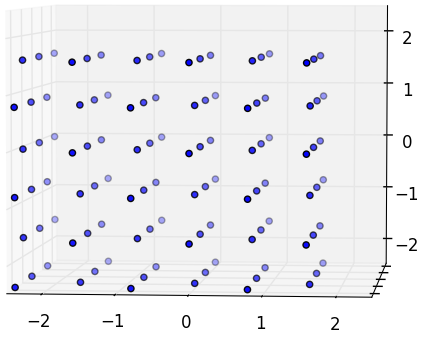
\includegraphics[scale=0.5]{fcc.png}
\caption{Initial placement of particles in FCC lattice }
\label{fig:init_place}
\end{figure}

Further some simulations were made to study argon in the the gas, liquid and solid phase. From the correlation function it can be easily seen in which phase the argon is  in. Thus in the following sections we will show results that has been achieved for the gas, liquid and solid phase.

\section{Microcanonical ensemble}

To control that we had a microcanonical ensemble we verified that the total energy of the system is constant after the equilibration. This is indeed seen in figure \ref{fig:all_rho}.

\begin{figure}[H]
\centering
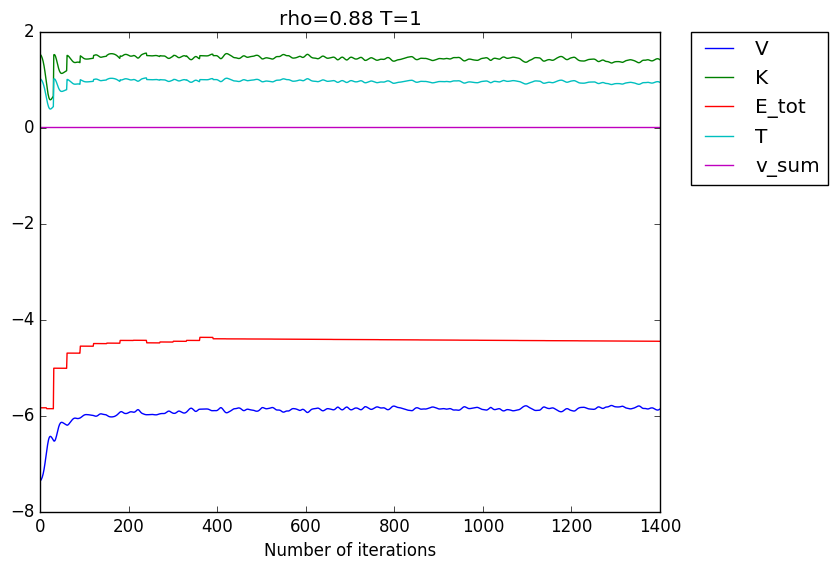
\includegraphics[scale=0.5]{All_rho088_T1_rm35_2.png}
\caption{The potential energy (blue) and kinetic energy (green) both fluctuate, but in opposing direction, leading to a constant total energy (red).}
\label{fig:all_rho}
\end{figure}

\section{Correlation function}

The correlation function for the gas phase are showed in figure \ref{fig:gas_cor}. From this figure it is evident that system is in the gas phase because the system doesn't exhibit any apparent structure. In the liquid phase it exhibits some structure, which is shown in figure \ref{fig:liq_cor}. A solid on the other hand, has a very clear lattice structure, as seen in \ref{fig:solid_cor}.

\begin{figure}[H]
\centering
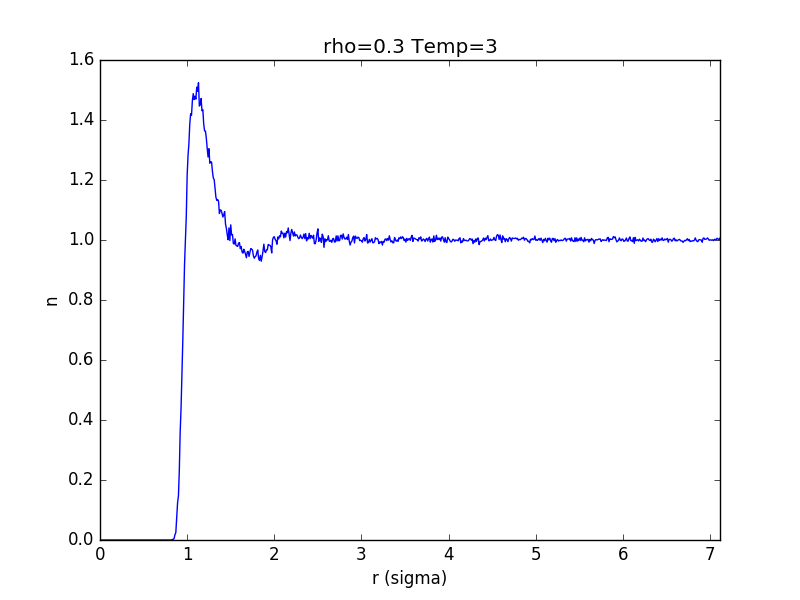
\includegraphics[scale=0.5]{Correlation_rho03_T3_rm35_2.png}
\caption{Spatial correlation function for $\rho=0.3$ and $T=3$ thus system is in the gas phase}
\label{fig:gas_cor}
\end{figure}

\begin{figure}[H]
\centering
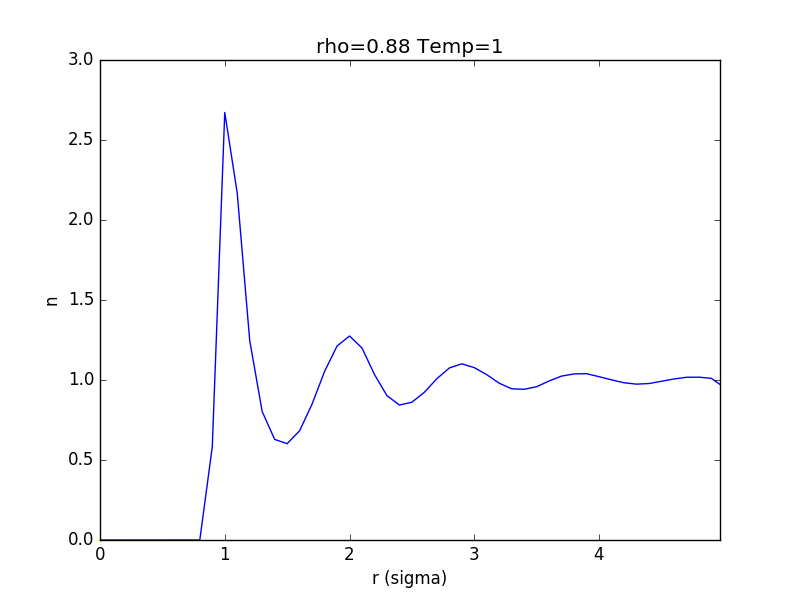
\includegraphics[scale=0.5]{Correlation_rho088_T1_rm35_2.png}
\caption{Spatial correlation function for $\rho=0.88$ and $T=1$ thus system is in the liquid phase}
\label{fig:liq_cor}
\end{figure}

\begin{figure}[H]
\centering
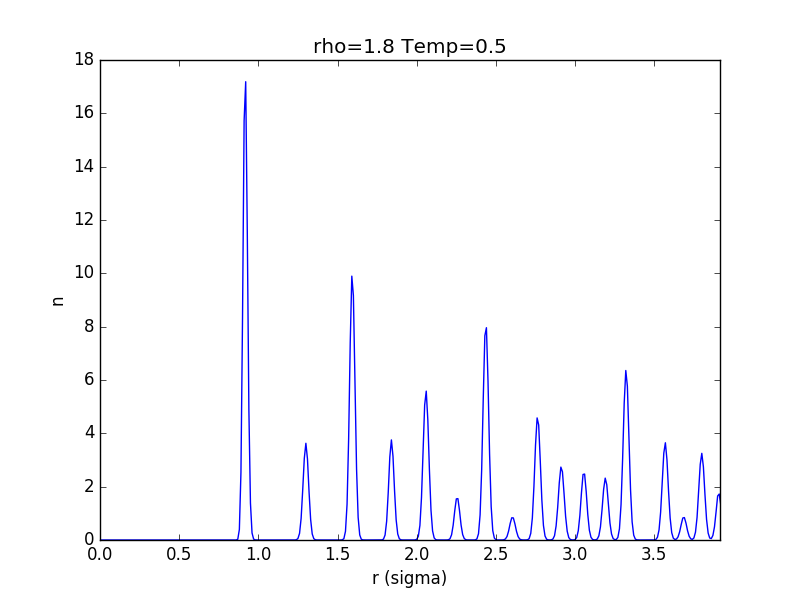
\includegraphics[scale=0.5]{Correlation_rho18_T05_rm35_2.png}
\caption{Spatial correlation function for $\rho=1.8$ and $T=0.5$ and the structure shows that this is a solid}
\label{fig:solid_cor}
\end{figure}

\section{Isothermals}

We can further investigate the phase of the system by generate isothermal lines in a $P$-$v$ plot. This is done by measuring the pressure while changing the density of the system and forcing a constant temperature using the thermostat. The resulting isothermals can be seen in figure \ref{fig:isothermals}. It is clear that for higher temperatures, the line becomes smoother and the dip disappears. The dip indicates that the system is undergoing a phase transition.

\begin{figure}[H]
\centering
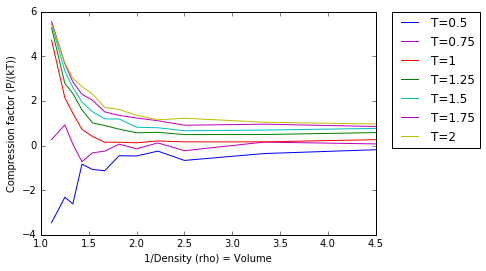
\includegraphics[scale=0.5]{Isothermen.png}
\caption{Isothermals for different temperatures. Note the absence of the dip for higher temperatures, indicating that the system is in gas phase.}
\label{fig:isothermals}
\end{figure}

\section{Diffusion}

We have also investigated the diffusion of particles in the system.
By keeping track of the displacement of each particle $x = |\mathbf{r}-\mathbf{r_0}|$ we can determine the diffusion coefficient $D$ using eq. \ref{eq:diffusion}. The result for different temperatures can be seen in fig. \ref{fig:diffusion}. It is clear that the diffusion coefficient of the gas is by far the largest, since the particles can move while barely interacting with others (ideal gas limit). On the other hand, the diffusion coefficient of the solid is practically nonexistent, since in that case the particles are bound to their position in the lattice.

\begin{equation}\label{eq:diffusion}
	<x^2> = D t
\end{equation}

\begin{figure}[H]
\centering
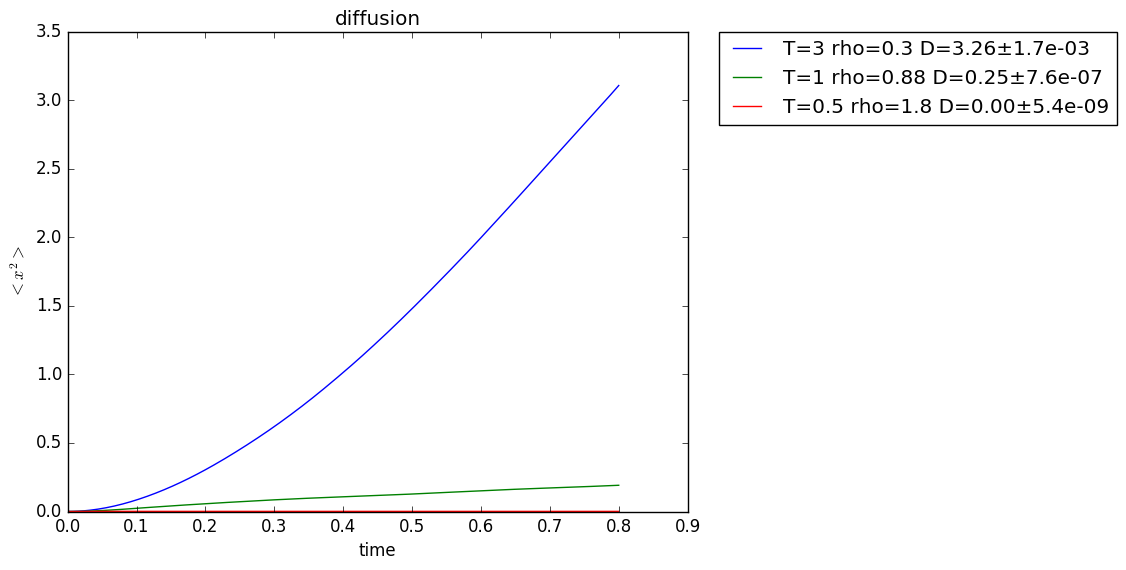
\includegraphics[scale=0.5]{diffusion.png}
\caption{Mean-square diffusion distance $<x^2>$ as function of time for a gas (blue), liquid (green) and solid (red). The slope is the diffusion coefficient $D$.}
\label{fig:diffusion}
\end{figure}

\section{Error analysis}

There were different methods used to determine the error in the pressure and the heat capacity. Firstly the error in the pressure was determined by measuring the pressure over each 100 steps over the course of one simulation after equilibration, and thereafter the variance in these values were used as the error for the pressure. Secondly to determine the error in the heat capacity the simulation was ran 5 times and for each of these 5 times the heat capacity was calculated and the variance in these values were used as the error for the heat capacity.

\chapter{Conclusion}

By comparing our results with other simulations performed that has been tested experimentally it can be concluded that this molecular dynamics simulation yields the desired results for argon. As shown in table \ref{table:results} these results corresponds to values that was given by \cite{thijssen} (table 8.1). We mostly compared the compression factor of our simulation.

Further we controlled the initial placement and the periodic boundary condition of the particles with an animation plot. Then we verified that we were measuring in the microcanonical ensemble by verifying that the total energy remained constant after the system was equilibrated. Hereafter the argon simulation was simulated in the gas, solid and liquid phase and this was checked by studying the correlation function of the system. And as was expected the correlation function of a solid and liquid appeared structured whereas the function of the gas had no structure to it. Moreover the heat capacity results were in accordance 
with previously performed experiments by Lebowitz \cite{lebowitz1967}. 

Also we studied isothermal lines in a PV diagram and compared these with the spatial correlation function to study phase "transitions" from a PV diagram. " sebas moet voegen" "zet eventueel problemen met isothermen op".


\newpage
\begin{thebibliography}{9}

\bibitem{thijssen}
 J.M. Thijssen (2007)\\
 $\textit{Computational Physics}$.\\
 Cambridge University Press
 
 \bibitem{lebowitz1967}
 Lebowitz, J. L. and Percus, J. K. and Verlet, L. (1967)\\
 $\textit{Ensemble Dependence of Fluctuations with Application to Machine Computations}$.\\
 American Physical Society
 \end{thebibliography}

\end{document}
